\documentclass[conference]{IEEEtran}
\IEEEoverridecommandlockouts
% The preceding line is only needed to identify funding in the first footnote. If that is unneeded, please comment it out.
\usepackage{cite}
\usepackage{amsmath,amssymb,amsfonts}
\usepackage{algorithmic}
\usepackage{graphicx}
\usepackage{textcomp}
\usepackage{xcolor}
\usepackage{listings}                           %顯示code用的
\usepackage{fontspec}                           %設定字體
\usepackage[CheckSingle, CJKmath]{xeCJK}
\usepackage{CJKulem}
\usepackage{listings}
\usepackage{color} %red, green, blue, yellow, cyan, magenta, black, white
\usepackage{float}

\definecolor{mygreen}{RGB}{28,172,0} % color values Red, Green, Blue
\definecolor{mylilas}{RGB}{170,55,241}

\setmainfont{Consolas}
%\setmonofont{Ubuntu Mono}
\setmonofont{Consolas}
\setCJKmainfont{Noto Sans CJK TC}
\XeTeXlinebreaklocale "zh"                      %中文自動換行

\lstset{language=Matlab,%
    %basicstyle=\color{red},
    breaklines=true,%
    morekeywords={matlab2tikz},
    keywordstyle=\color{blue},%
    morekeywords=[2]{1}, keywordstyle=[2]{\color{black}},
    identifierstyle=\color{black},%
    stringstyle=\color{mylilas},
    commentstyle=\color{mygreen},%
    showstringspaces=false,%without this there will be a symbol in the places where there is a space
    numbers=left,%
    numberstyle={\tiny \color{black}},% size of the numbers
    numbersep=9pt, % this defines how far the numbers are from the text
    emph=[1]{for,end,break},emphstyle=[1]\color{red}, %some words to emphasise
    %emph=[2]{word1,word2}, emphstyle=[2]{style},    
}

\def\BibTeX{{\rm B\kern-.05em{\sc i\kern-.025em b}\kern-.08em
    T\kern-.1667em\lower.7ex\hbox{E}\kern-.125emX}}

\begin{document}
\title{Digital Image Processing-Assignment 03\\
% {\footnotesize \textsuperscript{*}Note: Sub-titles are not captured in Xplore and should not be used}
% \thanks{Identify applicable funding agency here. If none, delete this.}
}

\author{\IEEEauthorblockN{1\textsuperscript{st} Zih Jie Lin}
\IEEEauthorblockA{\textit{Computer Science Information Engineering.} \\
\textit{Fu Jen Catholoic University}\\
New Taipei City, Taiwan \\
406261597@gapp.fju.edu.tw}
}
% \and
% \IEEEauthorblockN{2\textsuperscript{nd} Given Name Surname}
% \IEEEauthorblockA{\textit{dept. name of organization (of Aff.)} \\
% \textit{name of organization (of Aff.)}\\
% City, Country \\
% email address or ORCID}
% \and
% \IEEEauthorblockN{3\textsuperscript{rd} Given Name Surname}
% \IEEEauthorblockA{\textit{dept. name of organization (of Aff.)} \\
% \textit{name of organization (of Aff.)}\\
% City, Country \\
% email address or ORCID}
% \and
% \IEEEauthorblockN{4\textsuperscript{th} Given Name Surname}
% \IEEEauthorblockA{\textit{dept. name of organization (of Aff.)} \\
% \textit{name of organization (of Aff.)}\\
% City, Country \\
% email address or ORCID}
% \and
% \IEEEauthorblockN{5\textsuperscript{th} Given Name Surname}
% \IEEEauthorblockA{\textit{dept. name of organization (of Aff.)} \\
% \textit{name of organization (of Aff.)}\\
% City, Country \\
% email address or ORCID}
% \and
% \IEEEauthorblockN{6\textsuperscript{th} Given Name Surname}
% \IEEEauthorblockA{\textit{dept. name of organization (of Aff.)} \\
% \textit{name of organization (of Aff.)}\\
% City, Country \\
% email address or ORCID}

\maketitle

% \begin{abstract}
% \end{abstract}

% \begin{IEEEkeywords}
% \end{IEEEkeywords}

\section{實驗說明}
Apply Fourier transform to Lena image via ILPF,GLPF, and BLPF with n=1. Discuss the difference of results among each filter.

\section{程式碼}
\lstinputlisting{problem.m}

\section{成果}
原圖

\begin{figure}[H]
\centerline{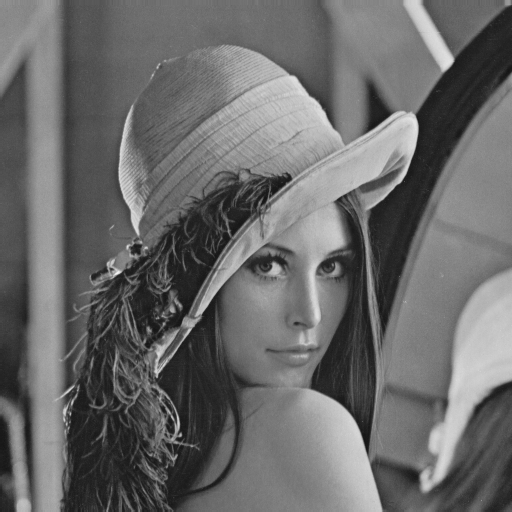
\includegraphics[width=6cm]{lena.png}}
\caption{lena}
\label{lena}
\end{figure}

\subsection{ILPF}

\begin{figure}[H]
\centerline{
\includegraphics[width=6cm]{ILPF0_2.jpg}}
\caption{ILPF, $D_0$ = $0.2$}
\label{ILPF0.2}
\end{figure}

\begin{figure}[H]
\centerline{
\includegraphics[width=6cm]{ILPF0_4.jpg}}
\caption{ILPF, $D_0$ = $0.4$}
\label{ILPF0.4}
\end{figure}

\begin{figure}[H]
\centerline{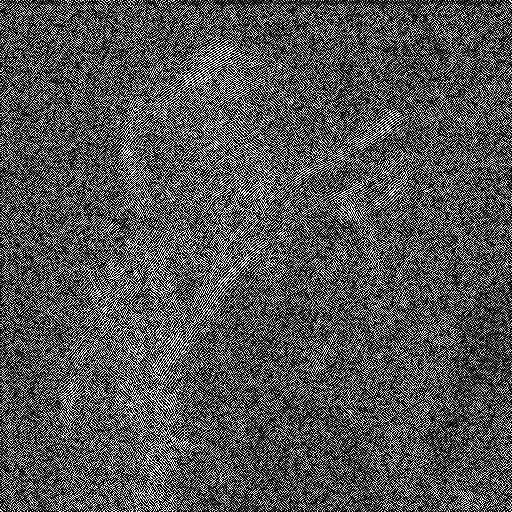
\includegraphics[width=6cm]{ILPF0_6.jpg}}
\caption{ILPF, $D_0$ = $0.6$}
\label{ILPF0.6}
\end{figure}

\begin{figure}[H]
\centerline{
\includegraphics[width=6cm]{ILPF0_8.jpg}}
\caption{ILPF, $D_0$ = $0.8$}
\label{ILPF0.8}
\end{figure}

\begin{figure}[H]
\centerline{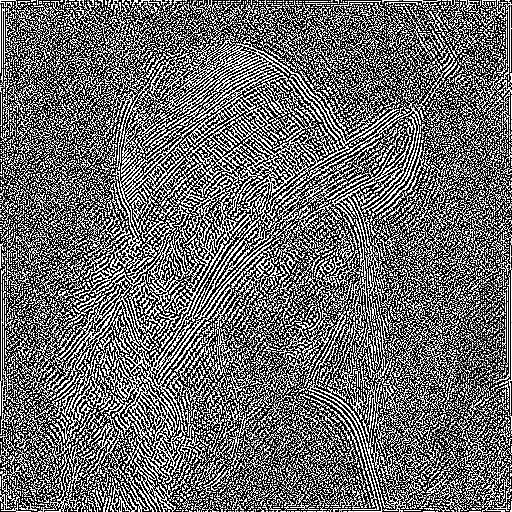
\includegraphics[width=6cm]{ILPF1_0.jpg}}
\caption{ILPF, $D_0$ = $1.0$}
\label{ILPF1.0}
\end{figure}

\begin{figure}[H]
\centerline{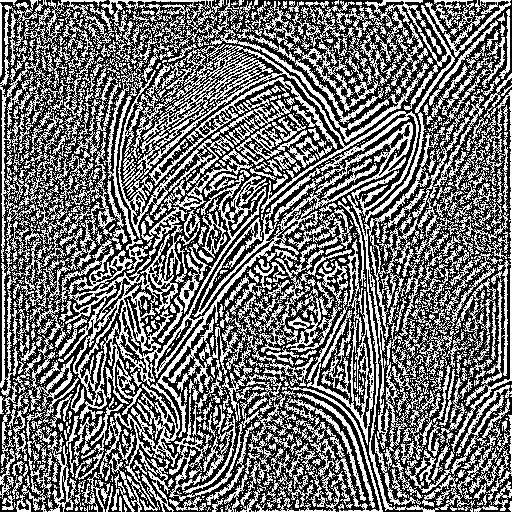
\includegraphics[width=6cm]{ILPF1_2.jpg}}
\caption{ILPF, $D_0$ = $1.2$}
\label{ILPF1.2}
\end{figure}

\begin{figure}[H]
\centerline{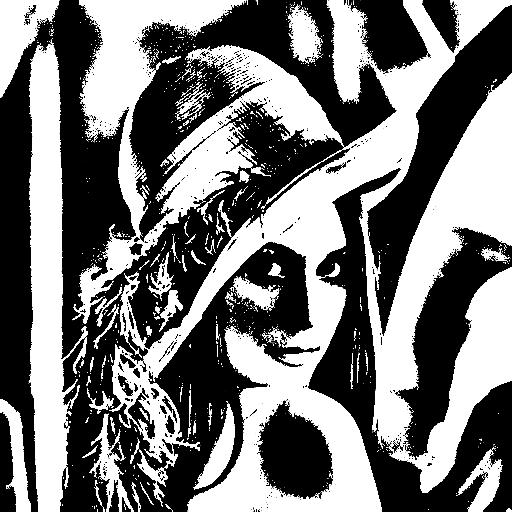
\includegraphics[width=6cm]{ILPF1_4.jpg}}
\caption{ILPF, $D_0$ = $1.4$}
\label{ILPF1.4}
\end{figure}

\subsection{GLPF}

\begin{figure}[H]
\centerline{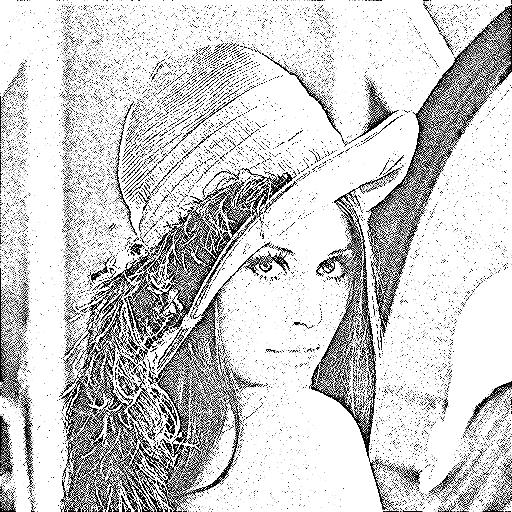
\includegraphics[width=6cm]{GLPF-0_5.jpg}}
\caption{GLPF, $D_0$ = $-0.5$}
\label{GLPF-0.5}
\end{figure}

\begin{figure}[H]
\centerline{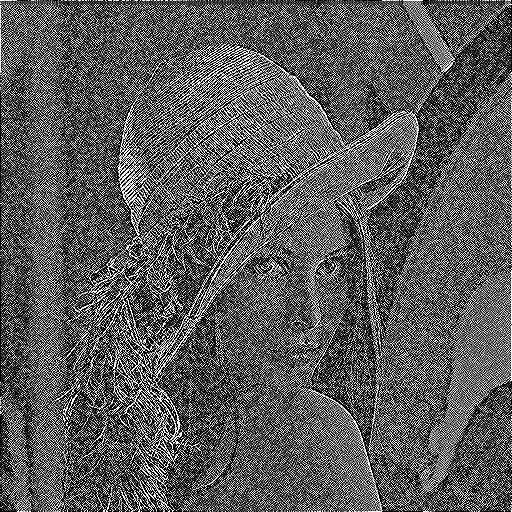
\includegraphics[width=6cm]{GLPF-0_4.jpg}}
\caption{GLPF, $D_0$ = $-0.4$}
\label{GLPF-0.4}
\end{figure}

\begin{figure}[H]
\centerline{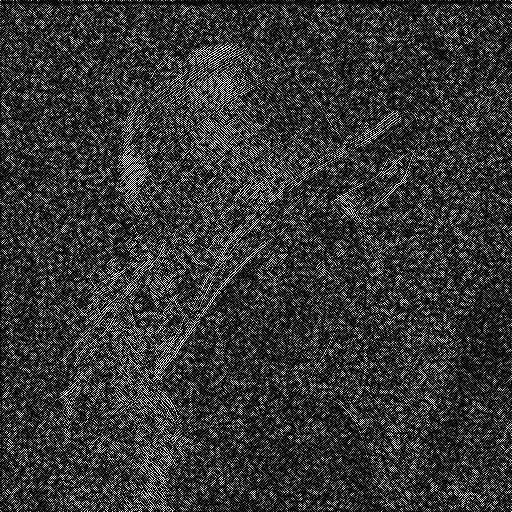
\includegraphics[width=6cm]{GLPF-0_3.jpg}}
\caption{GLPF, $D_0$ = $-0.3$}
\label{GLPF-0.3}
\end{figure}

\begin{figure}[H]
\centerline{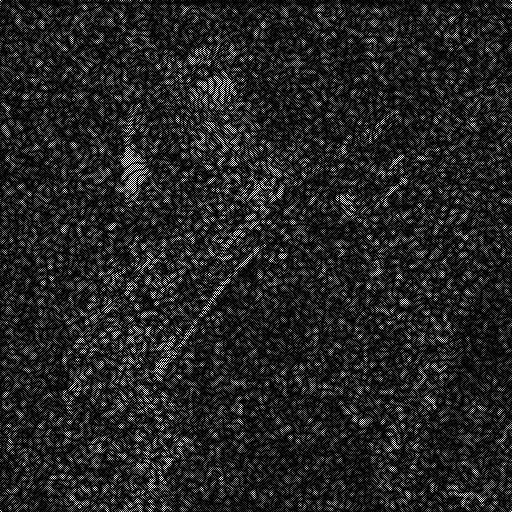
\includegraphics[width=6cm]{GLPF-0_2.jpg}}
\caption{GLPF, $D_0$ = $-0.2$}
\label{GLPF-0.2}
\end{figure}

\begin{figure}[H]
\centerline{
\includegraphics[width=6cm]{GLPF-0_1.jpg}}
\caption{GLPF, $D_0$ = $-0.1$}
\label{GLPF-0.1}
\end{figure}

\begin{figure}[H]
\centerline{
\includegraphics[width=6cm]{GLPF0_0.jpg}}
\caption{GLPF, $D_0$ = $0.0$}
\label{GLPF0.0}
\end{figure}

\begin{figure}[H]
\centerline{
\includegraphics[width=6cm]{GLPF0_1.jpg}}
\caption{GLPF, $D_0$ = $0.1$}
\label{GLPF0.1}
\end{figure}

\begin{figure}[H]
\centerline{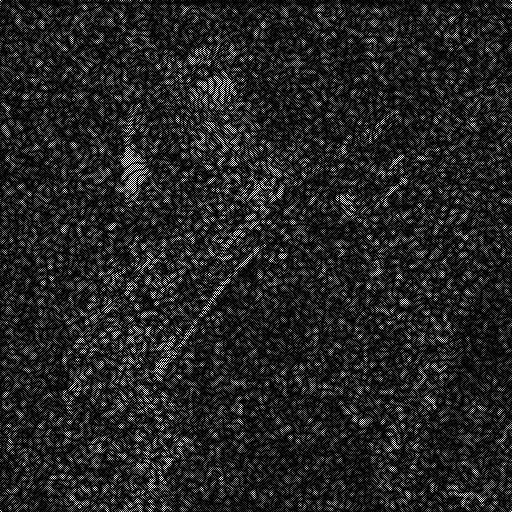
\includegraphics[width=6cm]{GLPF0_2.jpg}}
\caption{GLPF, $D_0$ = $0.2$}
\label{GLPF0.2}
\end{figure}


\begin{figure}[H]
\centerline{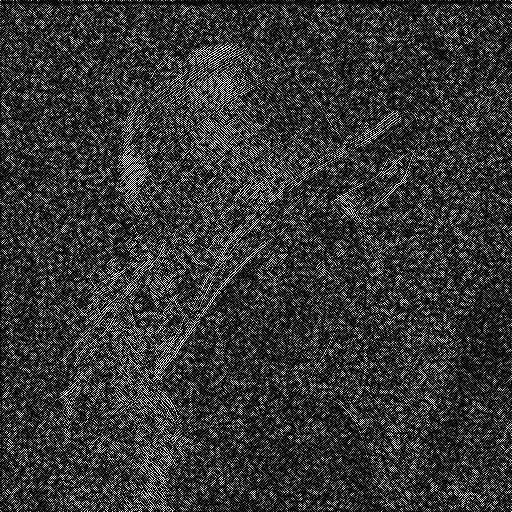
\includegraphics[width=6cm]{GLPF0_3.jpg}}
\caption{GLPF, $D_0$ = $0.3$}
\label{GLPF0.3}
\end{figure}

\begin{figure}[H]
\centerline{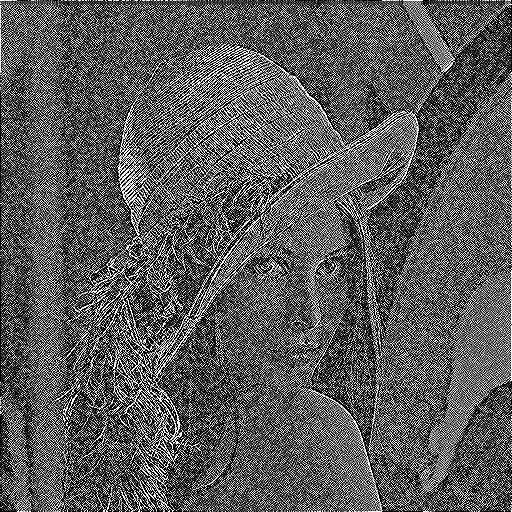
\includegraphics[width=6cm]{GLPF0_4.jpg}}
\caption{GLPF, $D_0$ = $0.4$}
\label{GLPF0.4}
\end{figure}

\begin{figure}[H]
\centerline{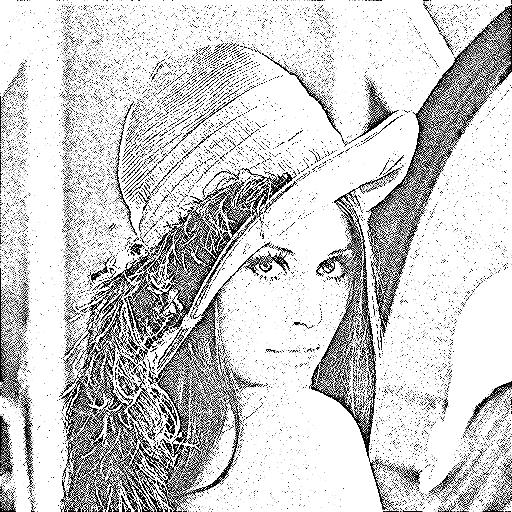
\includegraphics[width=6cm]{GLPF0_5.jpg}}
\caption{GLPF, $D_0$ = $0.5$}
\label{GLPF0.5}
\end{figure}


\subsection{BLPF}

\begin{figure}[H]
\centerline{
\includegraphics[width=6cm]{BLPF0.jpg}}
\caption{BLPF, $D_0$ = $0$}
\label{BLPF0}
\end{figure}

\begin{figure}[H]
\centerline{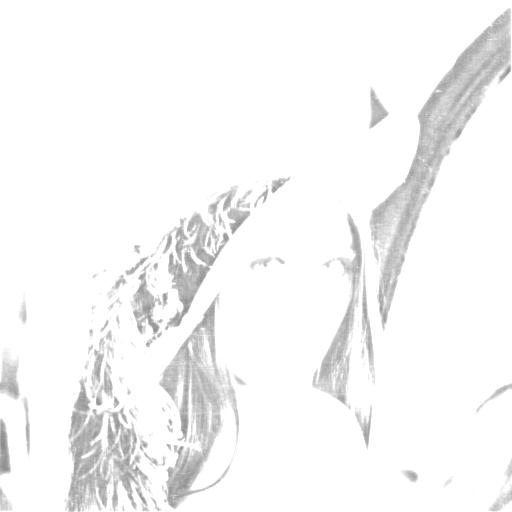
\includegraphics[width=6cm]{BLPF10.jpg}}
\caption{BLPF, $D_0$ = $10$}
\label{BLPF10}
\end{figure}

\begin{figure}[H]
\centerline{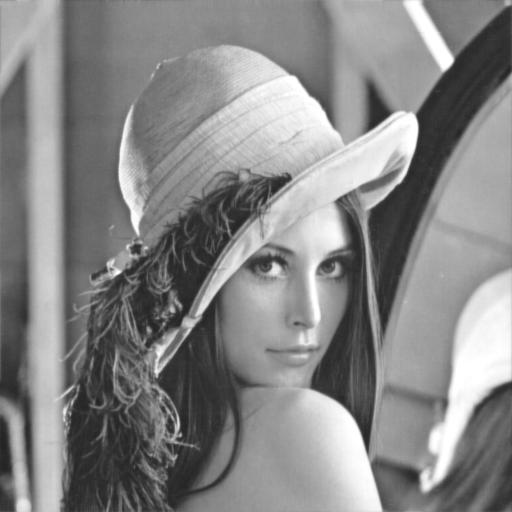
\includegraphics[width=6cm]{BLPF20.jpg}}
\caption{BLPF, $D_0$ = $20$}
\label{BLPF20}
\end{figure}

\begin{figure}[H]
\centerline{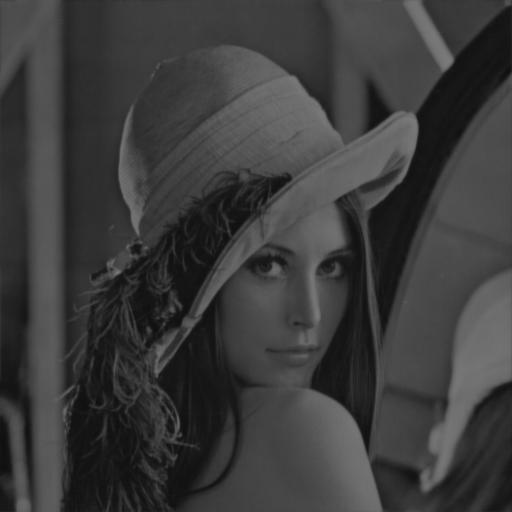
\includegraphics[width=6cm]{BLPF30.jpg}}
\caption{BLPF, $D_0$ = $30$}
\label{BLPF30}
\end{figure}

\begin{figure}[H]
\centerline{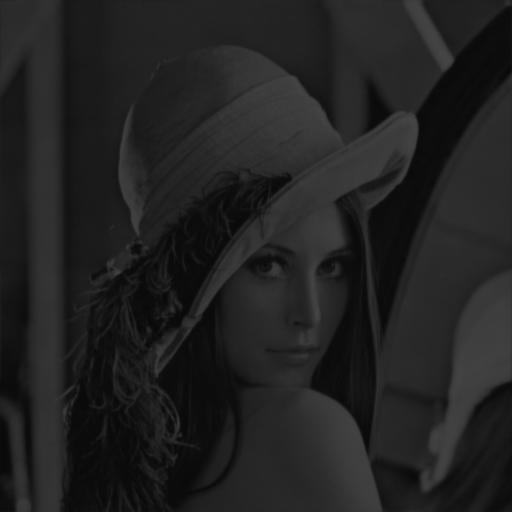
\includegraphics[width=6cm]{BLPF40.jpg}}
\caption{BLPF, $D_0$ = $40$}
\label{BLPF40}
\end{figure}

\begin{figure}[H]
\centerline{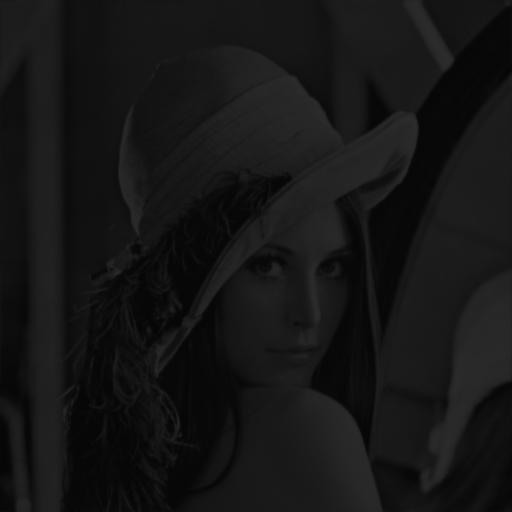
\includegraphics[width=6cm]{BLPF50.jpg}}
\caption{BLPF, $D_0$ = $50$}
\label{BLPF50}
\end{figure}

\section{比較}
ILPF 改變圖片的對比度,$D_0$ 越大,對比度越強烈,GLPF 改變圖片模糊程度,$D_0=x$ 或 $-x$ 的效果相同,$D_0$ 越大越模糊。BLPF 改變圖片明亮度,$D_0$ 越大,圖片越暗($D_0=0$ 除外)。

% % \begin{thebibliography}{00}
% % \end{thebibliography}

\vspace{12pt}

\end{document}
